% !TeX spellcheck = en_US
\documentclass[10pt,landscape]{article}
\usepackage{multicol}
\usepackage{calc}
\usepackage{ifthen}
\usepackage[landscape]{geometry}
\usepackage{hyperref}
\usepackage{amsmath, amsfonts, amssymb}
\usepackage{mathtools}
\usepackage {graphicx}
\usepackage {textcomp}

\usepackage{siunitx}
\usepackage{physics}

% English spacing
\usepackage{icomma}
\frenchspacing
\usepackage[english]{babel}
 \sisetup{output-decimal-marker = {.}}
 
 
% To make this come out properly in landscape mode, do one of the following
% 1.
%  pdflatex latexsheet.tex
%
% 2.
%  latex latexsheet.tex
%  dvips -P pdf  -t landscape latexsheet.dvi
%  ps2pdf latexsheet.ps



% This sets page margins to .5 inch if using letter paper, and to 1cm
% if using A4 paper. (This probably isn't strictly necessary.)
% If using another size paper, use default 1cm margins.
\ifthenelse{\lengthtest { \paperwidth = 11in}}
	{ \geometry{top=.5in,left=.5in,right=.5in,bottom=.5in} }
	{\ifthenelse{ \lengthtest{ \paperwidth = 297mm}}
		{\geometry{top=1cm,left=1cm,right=1cm,bottom=1cm} }
		{\geometry{top=1cm,left=1cm,right=1cm,bottom=1cm} }
	}

% Turn off header and footer
\pagestyle{empty}
 

% Redefine section commands to use less space
\makeatletter
\renewcommand{\section}{\@startsection{section}{1}{0mm}%
                                {-1ex plus -.5ex minus -.2ex}%
                                {0.5ex plus .2ex}%x
                                {\normalfont\large\bfseries}}
\renewcommand{\subsection}{\@startsection{subsection}{2}{0mm}%
                                {-1explus -.5ex minus -.2ex}%
                                {0.5ex plus .2ex}%
                                {\normalfont\normalsize\bfseries}}
\renewcommand{\subsubsection}{\@startsection{subsubsection}{3}{0mm}%
                                {-1ex plus -.5ex minus -.2ex}%
                                {1ex plus .2ex}%
                                {\normalfont\small\bfseries}}
\makeatother

% Don't print section numbers
\setcounter{secnumdepth}{0}


\setlength{\parindent}{0pt}
\setlength{\parskip}{0pt plus 0.5ex}

\newcommand{\extraline}{\vspace{1em}}
\newcommand{\halfline}{\vspace{0.5em}}
\newcommand{\deriv}{\ensuremath{\frac{d}{dx}}}
\newcommand{\tableindent}{\hspace{1.5em}}
\newcommand{\uvec}[1]{\ensuremath{{\hat{#1}}}}

% -----------------------------------------------------------------------

\begin{document}

\raggedright
\footnotesize
\begin{multicols}{3}

% multicol parameters
% These lengths are set only within the two main columns
%\setlength{\columnseprule}{0.25pt}
\setlength{\premulticols}{1pt}
\setlength{\postmulticols}{1pt}
\setlength{\multicolsep}{1pt}
\setlength{\columnsep}{2pt}

\begin{center}
     \Large{\textbf{Structure \& Bonding}} \\
     \small{Luke Zhou $\cdot$ CHM 2311 $\cdot$ Winter 2022}
\end{center}

\section{Atomic Structure \& Quantum Theory}

Wavelength, frequency and the speed of light
\[ c = \lambda\nu  = \SI{2.998E8}{\meter/\second}  \]

Energy quantization
\[E = \frac{hc}{\lambda} = h\nu  \qquad
 h = \SI{6.626E-34}{\joule\cdot\second}  \]

Energy emitted by a \underline{hydrogen} atom: Bohr model
 \[ \Delta E = E_{h} - E_{l} = R_H \left(  \frac{1}{n_l^2} - \frac{1}{n_h^2} \right) \] 
 \[ R_H =  \SI{2.179E-18}{\joule} \]

Hydrogen emission spectra series \\
\begin{tabular}{@{\tableindent}ll@{}}
	Lyman series & $n_l = 1$ \\
	Balmer series & $n_l = 2$ \\
	Paschen series & $n_l = 3$ \\
	Brackett series & $n_l = 4$ \\
	Pfund series & $n_l = 5$ \\
	Humphreys series & $n_l = 6$ \\
\end{tabular}
\extraline

Wave-Particle Duality  
\[  mv = \frac{h}{\lambda} \]


Heisenberg Uncertainty Principle
\[  \Delta x \Delta p \geq \frac{h}{4\pi} \]

Schrödinger Wave Equation
\[ H\Psi = E\Psi  \]
\[ \left[ \frac{-h^2}{8\pi^2m} +
V(x,y,z)\right] \Psi(x,y,z) = E\Psi(x,y,z)  \]
	
Particle in a box
\[ \Psi(x) = \sqrt{\frac{2}{a}} \sin\left( \frac{n\pi x}{a} \right)  \qquad n \in \mathbb{N} \]
\[ E = \frac{n^2h^2}{8ma^2} \]

Particle on a ring
\[ \Psi(x) = B \exp \left(\frac{in\pi x}{L} \right)
\qquad n \in \mathbb{Z}, L = n\lambda  \]
\[ E = \frac{h^2}{8mL^2} (2n)^2 \]

Hydrogenic wave functions
\[ \Psi(r,\theta,\phi) = R(r) Y(\theta,\phi) \]

\tableindent N.B. $R(r)$ is usually graphed against $r/a_0$


Quantum numbers 
\begin{tabular}{@{\tableindent}lllp{2.5cm}@{}}
$n$ & Principal & $1, 2, 3, 4, \ldots $ & \scriptsize{orbital size} \\
$l$ & Angular & $0, 1, 2 \dots  n-1 $ & \scriptsize{orbital shape} \\
$m_l$ & Magnetic & $0, \pm 1, \pm 2, \ldots \pm l $ & \scriptsize{orbital orientation} \\
$m_s$ & Spin & $-\frac{1}{2}, +\frac{1}{2} $ &  \scriptsize{angular momentum direction} \\
\end{tabular}

\extraline
\tableindent $l$ can also be described with the letters $s, p, d, f, g, \ldots$
\extraline

Radial \& angular nodes

\begin{tabular}{@{\tableindent}llp{2.4cm}@{}}
\# of radial nodes & $n-l-1$ & $R(r) = 0$ \scriptsize{(spheres)}\\
\# of angular nodes & $l$ &  $Y(\theta,\phi)=0$ \scriptsize{(planes, cones)} \\
Total \# of nodes & $n-1$ & 
\end{tabular}
\extraline

Electron configurations

\begin{tabular}{@{\tableindent}p{2.5cm}p{4.5cm}@{}}
Aufbau Principle & Fill lower energy levels first: 1s, 2s, 2p, 3s, 3p, \textbf{4s}, \textbf{3d}, 4p, 5s, 4d, 5p, \ldots\\
Pauli Exclusion Principle & No two e- can have the same set of quantum numbers. \\
Hund's Rule & Fill degenerate levels separately w/ spins parallel -- this minimizes the energies below \\
\end{tabular}
\extraline

Energies to be minimized

\begin{tabular}{@{\tableindent}p{25mm}p{47mm}@{}}
	Coulombic Energy of Repulsion & \textdownarrow{} e- pairing = \textdownarrow{} $E$ \\
	Exchange Energy & \textuparrow{} parallel spins in separate orbitals = \textdownarrow{} $E$
\end{tabular}


Magnetism

\begin{tabular}{@{\tableindent}lp{5cm}@{}}
Paramagnetism & Attracted by a magnetic field; elements w/ unpaired e- \\
Dimagnetism & Slightly repelled by a magnetic field; elements w/ no unpaired e-
\end{tabular}

Transition Metals
\begin{itemize}
\item In ionization, e- are first removed from orbitals w/ density farthest from nucleus; i.e. from $ns$ before $(n-1)s$
\item Half- and fully-filled shells minimize exchange energy \& e- pairing: e.g., Cr ([Ar]4s$^1$3d$^{5}$) \& Cu  ([Ar]4s$^1$3d$^{10}$) 
\item All $M^{2+}$ ions are 3d-only; e.g.,  Fe$^{2+}$ is [Ar]$3d^{6}4s^0$
%\& Fe ([Ar]$4s^23d^{6}$)
\end{itemize}  


Effective nuclear charge
\[ Z_\text{eff} = Z_\text{actual} - S \]

Slater's screening constant \& rules
\begin{enumerate}
\item List orbitals in groups, merging s \& p: (1s) (2s, 2p) (3s, 3p) (3d) (4s, 4p) (4d) (5s, 5p), \ldots 
\item For e- in $ns$ or $np$ orbitals:

	\begin{enumerate}
	\item Each e- in the same $ns$ or $np$ (i.e. same grouping) as the one of interest contributes 0.35 (except 1s: 0.30)
	\item Each in the $(n-1)$ level: 0.85
	\item Each in the $(n-2)$ levels or lower: 1.00
	\end{enumerate}

\item For e- in $nd$ or $nf$ orbitals:

	\begin{enumerate}
	\item Each e- in the same $nd$ or $nf$  orbital as the e- of interest contributes 0.35
	\item Each in the groupings to the left: 1.00
	\end{enumerate}

\end{enumerate}

Periodic trends

\begin{center}
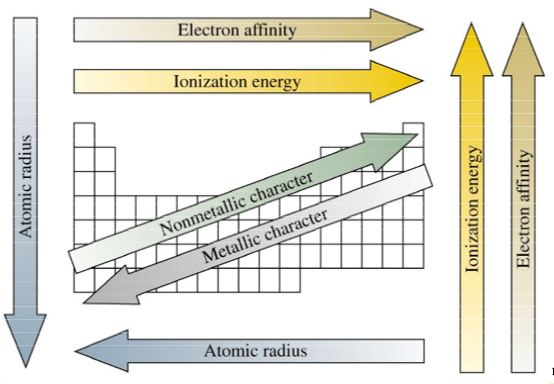
\includegraphics[width=\linewidth]{./chm2311/periodic-table-trends.png}
\end{center}
 
\begin{itemize} 
\item Atomic radius: size of outermost orbital containing e-. Larger $n$ or higher $Z_\text{eff}$ = lower radius.
\item Ionization energy: for removal of an e-. Always endothermic. Larger atomic radius  = lower IE.  Second IE is much higher than the first.
\item Electron affinity: energy in adding an e- to an isolated atom. Usually exothermic (i.e. negative). Larger atomic radius = less attraction to nucleus = less-negative EA. Second EA is always endothermic. 
\item Electronegativity: ability of a bonded atom to attracted shared electrons. EN is relative.
\end{itemize}

\hrulefill


\section{Constants}

Planck's constant
\[ h = \SI{6.626E-34}{\joule\cdot\second} \]
 
 Rydberg constant for hydrogen
 \[ R_H =  \SI{2.179E-18}{\joule} \]
 
Electron mass
\[  m_e = \SI{9,11E-31}{\kilogram} \]

Speed of light
\[ c = \SI{2.998E8}{\meter/\second}  \]

Bohr radius {(most probable dist b/w nucleus \& e- in a ground-state H atom)}
\[ a_0 = \SI{52.9}{\pico\metre} \]

Conversions
\[ \SI{1}{\metre} = 10^9 \, \si{\nano\metre} = 10^{12} \, \si{\pico\metre}\]
\[ \SI{1}{\joule} = \SI{1}{\kilogram\cdot\metre^2/\sec^2}  \]


\hrulefill

\section{Molecular Structure \& Bonding}

Types of bonding 

\begin{tabular}{@{\tableindent}llp{26mm}<{\raggedright}@{}}
	Covalent & $\text{EN}_A \sim  \text{EN}_B$ & Quantum (wave) mechanics \\
	Polar covalent & $\text{EN}_A < \text{EN}_B$ & \\
	Ionic & $\text{EN}_A \ll  \text{EN}_B$ &  Classic electrostatics \\
\end{tabular}

Lewis structures: formal charge
\[
\begin{pmatrix}
	 \text{\# of valence e-} \\
	 \text{in a free atom of} \\
	  \text{the element}
\end{pmatrix}
-
\begin{pmatrix}
	\text{\# of unshared} \\
	\text{e- on the atom} 
\end{pmatrix}
-
\begin{pmatrix}
	\text{\# of bonds} \\
	\text{to the atom} 
\end{pmatrix}
\]
\[ \text{Total charge on molecule or ion} = \text{sum of formal charges} \]

\extraline

Lewis structures: chemical properties

\begin{tabular}{@{\tableindent}lp{2.45cm}<{\raggedright}p{2.6cm}<{\raggedright}@{}}
Lewis base & Nucleophile (e- pair donor) & -ve formal charges \& lone pairs \\
Lewis acid & Electrophile (e- pair acceptor) & atoms lacking full octets
\end{tabular}
\extraline

VSEPR notation
\[ \text{AX}_n\text{E}_m \]
\tableindent (A: central atom, $n$: \# of bonding pairs, $m$: \# of lone pairs) \\
\extraline


VSEPR (Valence Shell Electron Pair Repulsion Theory): geometries \& shapes

\begin{tabular}{@{\tableindent}cp{0.3\linewidth}<{\raggedright}p{0.4\linewidth}<{\raggedright}@{}}
\textsc{Steric \#} & \textsc{Geometry} & \textsc{Shapes} \\ 
2 & Linear (180°) 
	& Linear \\
3 & Trigonal Planar (120°)
	& Trigonal Planar, Bent / V-shaped \\
4 & Tetrahedral (109.5°)
	& Tetrahedral, Trigonal Pyramidal, Bent / V-shaped  \\
5 & Trigonal Bipyramidal (120°, 90°)
	& Trigonal Bipyramidal, See-saw, T-shaped, Linear  \\
6 & Octahedral (90°)
	& Octahedral, Square Pyramidal, Square Planar \\
7 & Pentagonal Bipyramidal & \\ %(72°, 90°)
8 & Square Antiprismatic & \\ %(70,5°, 99,6°, 109,5°)
\end{tabular}
\extraline

Lone pair placement:  $\downarrow$ \# of nearest neighbours (in terms of angle)
\begin{itemize}
	\item Trigonal bipyramidal: LP occupy equatorial slots (so it has 2 axial nearest neighbours, 90° away) rather than axial (3 equatorial neighbours, 90° away)
	\begin{itemize}	
		\item Lower-EN atoms tend to prefer equatorial positions too
	\end{itemize}
	\item Octahedral: LP occupy axial slots (all neighbours 90° away)
\end{itemize}


VSEPR: degree of repulsion
\[ \text{BP/BP} < \text{BP/LP} < \text{LP/LP} \]
\[ \text{single bond} < \text{double bond} < \text{triple bond} < \text{lone pair} \]

VSEPR: bond angle trends for molecules with \underline{lone pairs}
\begin{itemize}
\item General principle: 
	\begin{itemize}
		\item  $\downarrow$ e- density on A = $\uparrow$ space occupied by LPs = $\downarrow$ repulsion b/w BP 
		\item $\therefore$ $\downarrow$ bond angles
	\end{itemize}

\item Central atom A: 
	\begin{itemize}
		\item $\downarrow$ EN  = $\downarrow$ e- density on A = $\downarrow$ bond angles
		\item $\uparrow$ size =  $\downarrow$ e- density on A = $\downarrow$ bond angles
		%\item $\uparrow$ bond length
	\end{itemize}

\item Terminal atoms X: 
	\begin{itemize}
		\item $\uparrow$ EN  = $\downarrow$ e- density on A = $\downarrow$ bond angles
		\item $\downarrow$ size = $\downarrow$ space needed by X = $\downarrow$ bond angles
		%\item $\downarrow$ bond length
	\end{itemize}
\end{itemize}

Dipole moments \\
\tableindent Direction: $\delta + \rightarrow \delta -$ (less EN $\rightarrow$ more EN) 
\extraline

Valence Bond Theory

\begin{tabular}{@{\tableindent}lp{16mm}p{42mm}@{}}
$\sigma$ bonds & single bonds & head-on overlap of hybridized orbitals \\
$\pi$ bonds & double/triple bonds & interactions b/w  remaining unhybridized orbitals \\
\end{tabular}
\extraline

Valence Bond Theory: Orbital hybridization 
%
\begin{tabular}{@{\tableindent}cll@{}}
	\textsc{Steric \#} & \textsc{Geometry} & \textsc{Hybridization} \\ 
	2 & Linear & (none) \\
	3 & Trigonal Planar 
	& $sp$ \\
	4 & Tetrahedral 
	& $sp^2$ \\
	5 & Trigonal Bipyramidal 
	& $sp^3$ \\
	6 & Octahedral 
	& $sp^3d$ \\
	7 & Pentagonal Bipyramidal & $sp^3d^2$ \\ 
	8 & Square Antiprismatic & $sp^3d^3$ \\
\end{tabular}
\extraline


\hrulefill

\section{Symmetry \& Group Theory}

%Symmetry elements: points, axes, planes
%\extraline

Symmetry operations
%
\renewcommand{\arraystretch}{1.4}
\begin{tabular}{@{\tableindent}cp{0.18\linewidth}<{\raggedright}p{0.6\linewidth}<{\raggedright}@{}}
	$E$ & Identity & No change \\
	$C_n$ & (Proper) rotation  & Rotation by $(360/n)$° about an axis of rotation \\
	$\sigma$ & Reflection  & Reflection through a mirror plane \\
	$i$ & Inversion  & Every point $(x, y, z) \rightarrow (-x, -y, -z)$ \\ %-- movement through the centre of the object to a position opposite and as far from the point as initially\\
	$S_n$ & Rotation-reflection (improper rotation)  & Rotation by $(360/n)$° followed by reflection through a plane \underline{perpendicular }to the axis of rotation
\end{tabular}
\renewcommand{\arraystretch}{1}

Types of reflection operations
%
\renewcommand{\arraystretch}{1.4}
\begin{tabular}{@{\tableindent}cp{0.2\linewidth}<{\raggedright}p{0.6\linewidth}<{\raggedright}@{}}
	$\sigma$ & Reflection & Reflection through a mirror plane (general symbol) \\
	$\sigma_h$ & ``Horizontal"  & Reflection through a mirror plane \underline{$\perp$ to the principle axis of rotation} \\
	$\sigma_v$ & ``Vertical" & Reflection through a mirror plane that \underline{includes the principle axis of} \underline{rotation} \\
	$\sigma_d$ & ``Dihedral" & Reflection through a mirror plane that \underline{bisects two $C_n'$ axes} \\
\end{tabular}
\renewcommand{\arraystretch}{1}

Other terms \& symbols
\renewcommand{\arraystretch}{1.4}
\begin{tabular}{@{\tableindent}lp{0,8\linewidth}@{}}
	$C_n$ & the principal axis; i.e. the $C_n$ w/ the highest order $n$ \\
	$C_n'$ & $\perp$ to principal axis \& passing thru several atoms \\
	$C_n''$ & $\perp$ to principal axis \& passing btwn outer atoms \\
\end{tabular}
\renewcommand{\arraystretch}{1}

Point group flow chart
\vspace{-1.5em}
\begin{center}
	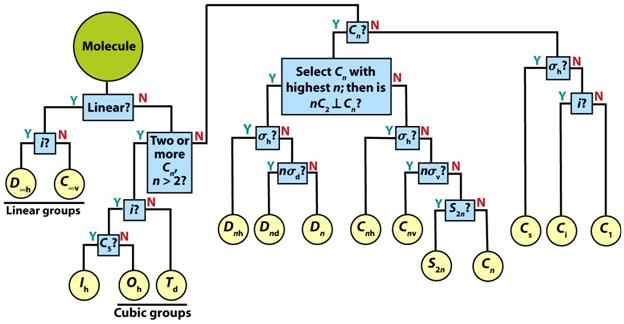
\includegraphics[width=\linewidth]{./chm2311/point-group-chart.jpeg}
\end{center}
\vspace{-1em}
\tableindent For the group $S_n$, $n$ must be even; otherwise, $S_n = C_{nh}$.
\extraline

Types of matrix representations for an operation
\begin{itemize}
	\item Matrix representation
	\item Irreducible representation
	\item Reducible representation ($\Gamma$ = $\sum$ of irreducible representation characters for the operation)
\end{itemize}

Characters in an irreducible representation
\begin{tabular}{@{\tableindent}ll@{}}
	1 & Symmetric w.r.t the operation \\
	-1 & Antisymmetric w.r.t the operation \\
\end{tabular}

\tableindent N.B. We align the principle axis of rotation w/ the $z$-axis.
\extraline

Symmetry labels
%
\renewcommand{\arraystretch}{1.4}
\begin{tabular}{@{\tableindent}lp{0.76\linewidth}@{}}
	$A$ & Function is symmetric w.r.t. $n$-fold rotation about main axis. \\
	$B$ & Function is anti-symmetric w.r.t. $n$-fold rotation about main axis. \\
	$E, T$ & Degenerate functions (interconvert with symmetry operations): doubly \& triply, respectively. \\
	1, 2 & Function is symmetric (or anti) w.r.t. $C_2'$ $\perp$ to principle axis, OR if missing, a $\sigma_v$ (specifically not $C_2''$ or $\sigma_v'$). \\
	$g, u$ & Function is symmetric (or anti) w.r.t. $i$. \\
	$'$, $''$ & Function is symmetric (or anti) w.r.t. $\sigma_h$. \\
	$\Sigma^+, \Sigma^-$ & Linear molecule symmetric (or anti) w.r.t. $\sigma_v$ \\
\end{tabular}
\renewcommand{\arraystretch}{1}
\medskip

Assigning symmetry labels to irreducible representations: go only as far as you need; i.e. until all have unique labels
\begin{enumerate}
	\item Look @ character of $E$ in the representation (row):
	\begin{itemize}
		\item If $\chi(E)=1$, label is $A$ if $C_n = 1$ and B if $C_n=-1$ ($C_n$: principle axis).
		\item If $\chi(E)=2$, label is $E$. 
		\item If $\chi(E)=3$, label is $T$. 
		\item $D_2$ and $D_{2h}$ have no principle axis; consider the sum of the characters of the $C_2$ axes instead.
		\item $D_{2d}$, $D_{4d}$, $D_{6d}$ have no principle axis; consider the sum of the characters of the $S_{2n}$ axes, not $C_n$
	\end{itemize}

	\item If label was $A$ or $B$ (not $E$ or $T$), consider the character of the $\perp C_2'$ axis (specifically containing outer atoms): 
	\begin{itemize}
		\item If $\chi(C_2')=1$, add subscript 1 to label.
		\item If $\chi(C_2')=-1$, add subscript 2 to label.
	\end{itemize}

	\item If $\nexists$ $C_2'$ (e.g., in point group $C_{nv}$), consider the character of the $\sigma_v$ (not $\sigma_v'$)
	\begin{itemize}
		\item If $\chi(\sigma_v)=1$, add subscript 1 to label.
		\item If $\chi(\sigma_v)=-1$, add subscript 2 to label.
	\end{itemize}

	\item If $\nexists$ $C_2', \sigma_v$, then we will not use subscripts 1 \& 2. (e.g., point groups $C_n, C_{nh}, S_{2n}$).
	
	\item Look @ character of $i$.
	\begin{itemize}
		\item If $\chi(i)=1$, add subscript $g$ (gerade) to label.
		\item If $\chi(i)=-1$, add subscript $u$ (ungerade) to label.
	\end{itemize}

	\item If more distinction needed, look @ character of $\sigma_h$.
	\begin{itemize}
		\item If $\chi(\sigma_h)=1$, add $'$ to label.
		\item If $\chi(\sigma_h)=-1$, add $''$ to label.
	\end{itemize}
\end{enumerate}

Characters for degenerate representations ($E, T$)
\begin{enumerate}
	\item Perform all \underline{unique} symmetry elements for each class.
	\begin{itemize}
		\item e.g., class $3C_2$ means do all three $C_2$ operations if they're non-coaxial; otherwise, just do one
		\item Apply the transformations to unit vectors.
	\end{itemize}
	\item Sum up all $x$ \& $y$ coordinates for the transformed points.
\end{enumerate}

Properties of character tables
\begin{enumerate}
	\item Order $h$: total \# of symmetry operations (e.g., $E$ and $3C_4$ make $h=4$)
	\item  Classes: total \# of symmetry operation \underline{types} (e.g., $E$ and $3C_4$ make order 2)
	\item \# irreducible representations (rows) = \# classes (columns)
	\item $\sum [\chi_i ]^2 = h$ for any irreducible representation
	\item Irreducible representations $A_i$ are all orthogonal to teach other: ${A_i} \cdot {A_j} = 0, i\neq j$ 
	\item All groups include a totally symmetric representation, with character 1 for all operations; this represents the $s$-orbital
\end{enumerate}

\hrulefill

\section{Molecular Orbital Theory}

Terms to know
\begin{itemize}
	\item Frontier MOs: Highest Occupied Molecular Orbitals (HOMO),  Lowest Unoccupied Molecular Orbitals (LUMO)
	\item Bonding vs. non-bonding interactions
	\item Side-to-side vs. end-to-end (head-to-head) vs. orthogonal interactions
	\item Constructive vs. destructive vs. zero interference
\end{itemize}



Bond order
\[
\begin{pmatrix}
	\text{bond} \\
	\text{order} 
\end{pmatrix}
= 
\frac{
	\frac{1}{2}
	\left[
		\begin{pmatrix}
			\text{\# of e- in } \\
			\text{bonding orbitals} 
		\end{pmatrix}
		-
		\begin{pmatrix}
			\text{\# of e- in } \\
			\text{antibonding orbitals} 
		\end{pmatrix}
	\right]
}{\text{\# of interations}}
\]

Second period diatomics: orbital order \underline{w/o orbital mixing}: $B_2, C_2, N_2$
\[ \sigma_g(2s) < \sigma_u^*(2s) < \mathbf{\sigma_g(2p) < \pi_u(2p)} < \pi_g^*(2p) < \sigma_u^*(2p) \]

Second period diatomics: orbital order \underline{w/ orbital mixing}: $O_2, F_2$
\[ \sigma_g(2s) < \sigma_u^*(2s) < \mathbf{\pi_u(2p) < \sigma_g(2p)} < \pi_g^*(2p) < \sigma_u^*(2p) \]

This ``crossing over" happens because as we walk across a period, $Z_\text{eff}$ increases, as does the $\Delta E$ between orbital types. When $\Delta E \leq \SI{13}{\electronvolt}$, $s$ and $p$ orbitals can mix.

Stronger bonds = more virational fine structure = more peaks in photoelectron spectroscopy graph

Things to remember when drawing molecular orbital (MO) diagrams
\begin{itemize}
	\item $\sigma$-bonds: 0 nodes b/w nuclei; $\pi$: 1 node; $\delta$: 2 nodes 
	\item Atomic orbitals (AOs) \& group orbitals (GOs) interact when $\Delta E \leq \SI{13}{\electronvolt}$
	\item For interacting AOs/GOs: $\downarrow \Delta E$ b/w AOs/GOs = $\uparrow \Delta E$ b/w bonding \& anti-bonding MOs
	\begin{itemize}
			\item Homonuclear diatomics: high separation b/w bonding and anti-bonding MOs
			\item Heteronuclear diatomics: lower separation b/w bonding and anti-bonding MOs
	\end{itemize}
	\item Bonding MOs: more like the lower-energy AO/GO in character
	\item Anti-bonding MOs: more like the higher-energy AO/GO in character
	\item When 3+ AOs/GOs interact: consider which atom contributes more AOs/GOs
	\item Total \# of MOs = Total \# of constituent AOs used
\end{itemize}

Terms relating to MOs
\begin{itemize}
	\item Linear combinations of atomic orbitals (LCAOs): $\Psi = c_a \psi_a \pm c_b \psi_b$
	\item Symmetry-adapted linear combinations (SALCs)
\end{itemize}

Steps in drawing MOs for large molecules
\begin{enumerate}
	\item Determine the point group of the molecule.
	\item Determine the point group for each of the central atom's orbitals, within the molecule's point group.
	\item Find the point group for each of the GOs (symmetry-adapted linear combinations of the orbitals; SALCs) 
	\item Combine AOs of the central atom to the GOs having suitable symmetry
\end{enumerate}


\hrulefill

\scriptsize

\href{https://github.com/zhouluke/PhysicsFormulas}{Typography}  \copyright\ 2022 Luke Zhou. \\
Based on the course CHM 2311 Winter 2022 at the University of Ottawa \\
\href{http://wch.github.io/latexsheet/}{Document template}  \copyright\ 2014 Winston Chang.


\end{multicols}
\end{document}
